\documentclass{standalone}
\usepackage{pgfplots}
\pgfplotsset{compat=1.18}

\begin{document}

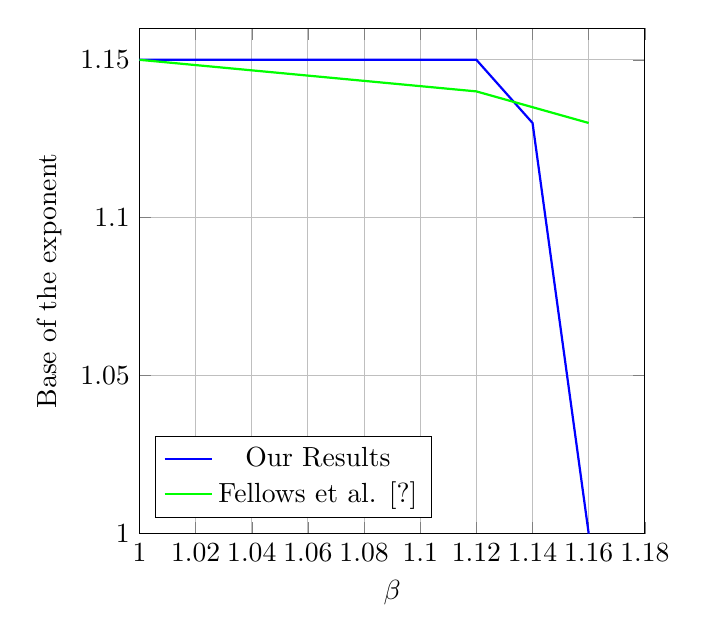
\begin{tikzpicture}
\begin{axis}[
    xlabel={$\beta$},
    ylabel={Base of the exponent},
    grid=both,
    xmin=1, xmax=1.18,
    ymin=1, ymax=1.16,
    legend pos=south west,
    width=8cm, height=8cm,
    tick label style={/pgf/number format/fixed},
    ytick={1, 1.05, 1.10, 1.15},
    xtick={1, 1.02, 1.04, 1.06, 1.08, 1.10, 1.12, 1.14, 1.16, 1.18}
]

\addplot[
    color=blue,
    thick
]
coordinates {
    (1, 1.15) (1.12, 1.15) (1.14, 1.13) (1.16, 1)
};

\addplot[
    color=green,
    thick
]
coordinates {
    (1, 1.15) (1.12, 1.14) (1.16, 1.13)
};

\legend{Our Results, Fellows et al. [?]}
\end{axis}
\end{tikzpicture}

\end{document}